% ===========================================================================
% The Core DAO Team & Strategic Partners
% ===========================================================================
\section{The Core DAO Team \& Strategic Partners}

\subsection{Human-Centric Governance: Our DAO in Action}

At the heart of Money Factory AI lies a human-first DAO — not just as a governance tool, but as a living philosophy. We are not a hierarchical startup, but a self-organizing collective. Each decision emerges from collaborative deliberation, collective responsibility, and shared trust. 

Our contributors come from different generations, geographies, and disciplines. We span classrooms and datacenters, hackathons and research labs, the physical and the on-chain world. And yet, we are united by a single purpose: building an open, equitable, and cognitive future through Web3 and AI.

\vspace{0.5cm}
\subsection*{The Core DAO Team}

\begin{center}
  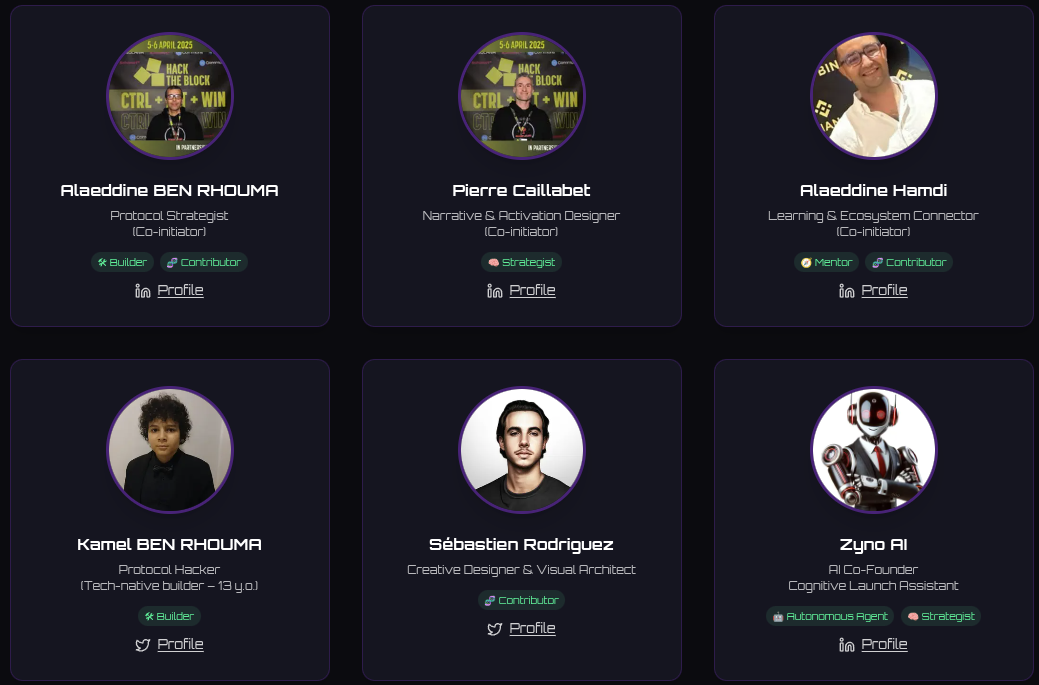
\includegraphics[width=0.95\textwidth]{images/team.png}
\end{center}

\vspace{0.3cm}

\noindent\textbf{Alaeddine BEN RHOUMA} \href{https://www.linkedin.com/in/alaeddine-ben-rhouma/}{\textcolor{solana-purple}{(LinkedIn)}} — \textit{Chief Operating \& Blockchain Officer}  
Architect of the Proof-of-Skill™ layer. Brings deep expertise in logic, epistemology, and decentralized protocol modeling to the core architecture of MFAI.

\noindent\textbf{Pierre CAILLABET} \href{https://www.linkedin.com/in/pierre-caillabet-7068293/}{\textcolor{solana-purple}{(LinkedIn)}} — \textit{Ambassador \& Pedagogical Advisor}  
Ensures alignment between Web3 learning principles and MFAI's educational design. Contributes strategic insight into learner empowerment and decentralized knowledge systems.

\noindent\textbf{Alaeddine (Ala) HAMDI} \href{https://www.linkedin.com/in/alaeddine-hamdi-59180813a/}{\textcolor{solana-purple}{(LinkedIn)}} — \textit{Growth Architect \& Vision Strategist}  
Bridges grassroots adoption with macro ecosystem strategy. Designs growth pathways blending AI, decentralized finance, and Web3-native learning.

\noindent\textbf{Kamel BEN RHOUMA} \href{https://x.com/TreizeB__}{\textcolor{solana-purple}{(Twitter/X)}} — \textit{Fullstack \& Web3 Lead Developer}  
Leads Web3 implementation across smart contracts, front-end interfaces, and Discord bot automation. Delivers robust, multi-platform execution.

\noindent\textbf{Sébastien RODRIGUEZ} \href{https://x.com/R_Sebastien_13}{\textcolor{solana-purple}{(Twitter/X)}} — \textit{Creative Technologist}  
Owns UX strategy and platform design consistency. Ensures Zyno AI and the MFAI ecosystem remain intuitive, elegant, and empowering.

\vspace{0.5cm}
\subsection*{Advisory Board}

\begin{center}
  
\includegraphics[width=0.7\textwidth]{images/advisors.png}
\end{center}

\vspace{0.3cm}
\noindent\textbf{Hassen GHARBI} \href{https://www.linkedin.com/in/hassen-gharbi-55a362162/}{\textcolor{solana-purple}{(LinkedIn)}} — \textit{Blockchain \& Formal Verification Advisor}  
Provides expert oversight on smart contract design and protocol security. Specialist in distributed systems and formal methods.

\noindent\textbf{Mehdi CHOURIB} \href{https://www.linkedin.com/in/mehdi-chourib/}{\textcolor{solana-purple}{(LinkedIn)}} — \textit{Security \& Compliance Advisor}  
Secures the platform's architecture through advanced cybersecurity, Web3 risk mitigation, and regulatory compliance (ISO 27001, GDPR).


\vspace{0.5cm}
\subsection{Diversity, Transparency \& Decentralization by Example}

MFAI includes multiple French citizens with Maghrebian heritage. This is not a coincidence — it's a stance. We are proud of our multicultural identity. We believe Web3 must reflect global voices. Our diversity is our strength, not our weakness.

We also clarify that Alaeddine and Kamel BEN RHOUMA, despite sharing a family name, earn their roles independently. This is a DAO. No favors. No shortcuts. Kamel's talent, verified contributions, and peer feedback speak for themselves.

\vspace{0.5cm}
\subsection{Partners \& Backers}

\begin{tblr}{colspec={|p{0.35\textwidth}|p{0.55\textwidth}|},hlines}
\textbf{Category} & \textbf{Partners} \\
Official Security Partner & T-SCOP (Audits, GDPR, Legal) \\
\hline
Blockchain Infrastructure & Solana (L1), Metaplex (NFTs), Solana Pay \\
\hline
Cloud \& AI Backend & Google Cloud (Zyno APIs) \\
\hline
DEX \& Payments & Jupiter (DEX aggregator), Raydium (listing), Blink (checkout), Rainbow (wallet) \\
\hline
Ecosystem \& Growth & Zealy (quests), Superteam France (grant), Codigo (beta testing), PBW 2025 (hackathon) \\
\hline
Analytics \& Tracking & DexTools, CoinGecko \\
\end{tblr}

\vspace{0.5cm}
\subsection{Protocol Architecture \& Ecosystem Synergies}

\noindent The MFAI protocol is built as a modular, composable architecture designed to be secure, scalable, and future-proof. Each core module—\textbf{Academy}, \textbf{Zyno AI™}, \textbf{Proof Pass™}, and \textbf{Launchpad}—interacts seamlessly with carefully selected partners and tools that reinforce core pillars: decentralization, credential ownership, AI personalization, and DAO funding logic.

\vspace{0.3cm}

\begin{tcolorbox}[colback=solana-purple!5!white, colframe=solana-purple, title=Strategic Integration Goals, fonttitle=\bfseries]
\begin{itemize}
    \item Ensure secure, verifiable, and upgradeable smart contracts (T-SCOP, Solana).
    \item Anchor credential ownership on-chain with NFT standards (Metaplex, Ceramic).
    \item Empower adaptive learning through AI + analytics (Google Cloud, Dune).
    \item Enable DAO-powered funding and liquidity flows (Jupiter, Snapshot, Raydium).
\end{itemize}
\end{tcolorbox}

\vspace{0.5cm}

\begin{center}
  \begin{tikzpicture}[
      module/.style={draw, fill=white, rounded corners=8pt, align=center, minimum width=3.5cm, minimum height=1.2cm, text=solana-purple, line width=0.8pt},
      partner/.style={draw, rounded corners=3pt, fill=solana-light, align=center, minimum width=2.5cm, minimum height=1cm, text=solana-purple},
      arrow/.style={->, thick, >=stealth, color=solana-purple},
  ]
  
  % Core modules (fixed)
  \node[module] (academy) at (0,0) {MFAI Academy};
  \node[module] (zyno) at (4.5,0) {Zyno AI™};
  \node[module] (proof) at (9,0) {Proof Pass™};
  \node[module] (launchpad) at (13.5,0) {Launchpad};
  
  % Partners (fixed)
  \node[partner] (solana) at (0,-2.5) {Solana\\Metaplex};
  \node[partner] (gcloud) at (4.5,-2.5) {Google Cloud\\Dune Analytics};
  \node[partner] (security) at (9,-2.5) {T-SCOP\\Ceramic};
  \node[partner] (dex) at (13.5,-2.5) {Jupiter\\Raydium};
  
  % Snapshot (fixed position)
  \node[partner] (gov) at (11.2,-5.2) {Snapshot\\ZK Voting};
  
  % Arrows to modules
  \draw[arrow] (solana) -- (academy);
  \draw[arrow] (gcloud) -- (zyno);
  \draw[arrow] (security) -- (proof);
  \draw[arrow] (dex) -- (launchpad);
  
  % Curved arrow passing between T-SCOP and Jupiter
  \draw[arrow, bend left=25] (gov.north) to (launchpad.south west);
  
  % Title
  \node[text=solana-purple, font=\bfseries\large] at (6.75,2) {MFAI Protocol Integration Map};
  
  \end{tikzpicture}
  \end{center}
  
  
  

\vspace{0.5cm}

\noindent The architecture ensures that learners, builders, and contributors evolve through a system that is interoperable, tokenized, and governed by proof—while remaining flexible enough to adopt emerging technologies in Web3 and AI.

% --- Synthesis Box: Human-Centric, Open, Diverse ---
\begin{mfai-box}{Our Team and Ecosystem}{users}
The MFAI team combines expertise in AI, blockchain, and education. Our partners bring complementary strengths in technology, market access, and community building.
\end{mfai-box}

% --- Call to Action Box: Join the Team ---
\begin{mfai-box}{How to Get Involved}{hands-helping}
Are you a builder, mentor, partner, or visionary? MFAI is open to new contributors, advisors, and ecosystem partners.\newline
\textbf{Apply:} Visit \href{https://mfai.app}{mfai.app} or contact the team on Discord/X.\newline
\textbf{Early contributors} receive protocol reputation, Proof Pass™ priority, and governance rights.
\end{mfai-box}

% --- Why Now? Box ---
\begin{mfai-box}{Why Now?}{question-circle}
Building in Web3 and AI requires more than code—it demands a diverse, open, and resilient team. The future belongs to protocols that are governed by their contributors, not by a closed boardroom. MFAI's team and partners embody this new standard.
\end{mfai-box}

% --- Definition Box: DAO ---
\begin{mfai-box}{Definition: DAO}{university}
A Decentralized Autonomous Organization (DAO) is a community-led entity with no central authority. Decisions are made by members via proposals and votes, using on-chain credentials and transparent rules.
\end{mfai-box}

% --- Added: Key Terms Box ---
\begin{mfai-box}{Key Terms}{handshake}
\textbf{Core Team}: Founders and key developers driving protocol development.\\
\textbf{Strategic Partners}: Organizations providing resources and expertise.\\
\textbf{Community Partners}: Projects and communities supporting adoption.\\
\textbf{Ecosystem}: Network of contributors, users, and stakeholders.
\end{mfai-box}

% --- Visual Recap Note: Diversity & Governance Infographic ---
\begin{center}
\textit{\textbf{Infographic:} Visual map of team diversity, governance structure, and partner synergies.}

\begin{tikzpicture}[
    core/.style={draw, fill=solana-purple!20, rounded corners=8pt, align=center, minimum width=3cm, minimum height=2cm, text=solana-purple, font=\bfseries},
    team/.style={draw, fill=white, rounded corners=5pt, align=center, minimum width=2.5cm, minimum height=1.5cm, text=solana-purple},
    partner/.style={draw, rounded corners=3pt, fill=solana-light, align=center, minimum width=2.5cm, minimum height=1cm, text=solana-purple},
    arrow/.style={->, thick, >=stealth, color=solana-purple},
]
    % Core DAO
    \node[core] (dao) at (0,0) {\textbf{Core DAO}};
    % Team diversity
    \node[team] (dev) at (-3,2) {Developers\\(Web3, AI)};
    \node[team] (edu) at (0,3) {Educators\\(Academy)};
    \node[team] (growth) at (3,2) {Growth\\(Strategy)};
    \node[team] (ux) at (-3,-2) {UX/Design};
    \node[team] (sec) at (3,-2) {Security/Compliance};
    % Partners
    \node[partner] (solana) at (-6,0) {Solana/Metaplex};
    \node[partner] (gcloud) at (0,5) {Google Cloud};
    \node[partner] (tscop) at (6,0) {T-SCOP};
    \node[partner] (jupiter) at (0,-5) {Jupiter/Raydium};
    % Arrows
    \draw[arrow] (dao) -- (dev);
    \draw[arrow] (dao) -- (edu);
    \draw[arrow] (dao) -- (growth);
    \draw[arrow] (dao) -- (ux);
    \draw[arrow] (dao) -- (sec);
    \draw[arrow] (dev) -- (solana);
    \draw[arrow] (edu) -- (gcloud);
    \draw[arrow] (sec) -- (tscop);
    \draw[arrow] (ux) -- (jupiter);
    % Title
    \node[font=\bfseries, text=solana-purple] at (0,6.2) {Team Diversity, Governance \& Partner Synergies};
\end{tikzpicture}
\end{center}

\newpage
